%\graphicspath{./Chapters/appendix1/figs/}


In this section I will describe the background and the current status of the fusion energy research related to this PhD thesis.
\section{Fusion energy} \label{Fusion_energy}

In a fusion reaction two light nuclei fuse and a heavier nucleus is generated. The energy released in the reaction depends on how strongly protons and neutrons are bound in the nucleus of reactant and products. This strength is expressed by the average binding energy per nucleon, that is the energy necessary to decompose one nucleus divided by the number of nucleons. The energy released by the nuclear reaction is given by the difference of the total binding energy in the products minus the reactants. \autoref{fig:binding_energy} shows that it is possible to obtain energy in two ways: fusion and fission. In fusion, the lighter the reactants the larger the energy released per nucleon tends to be.

\begin{figure}[!ht]
	\centering
	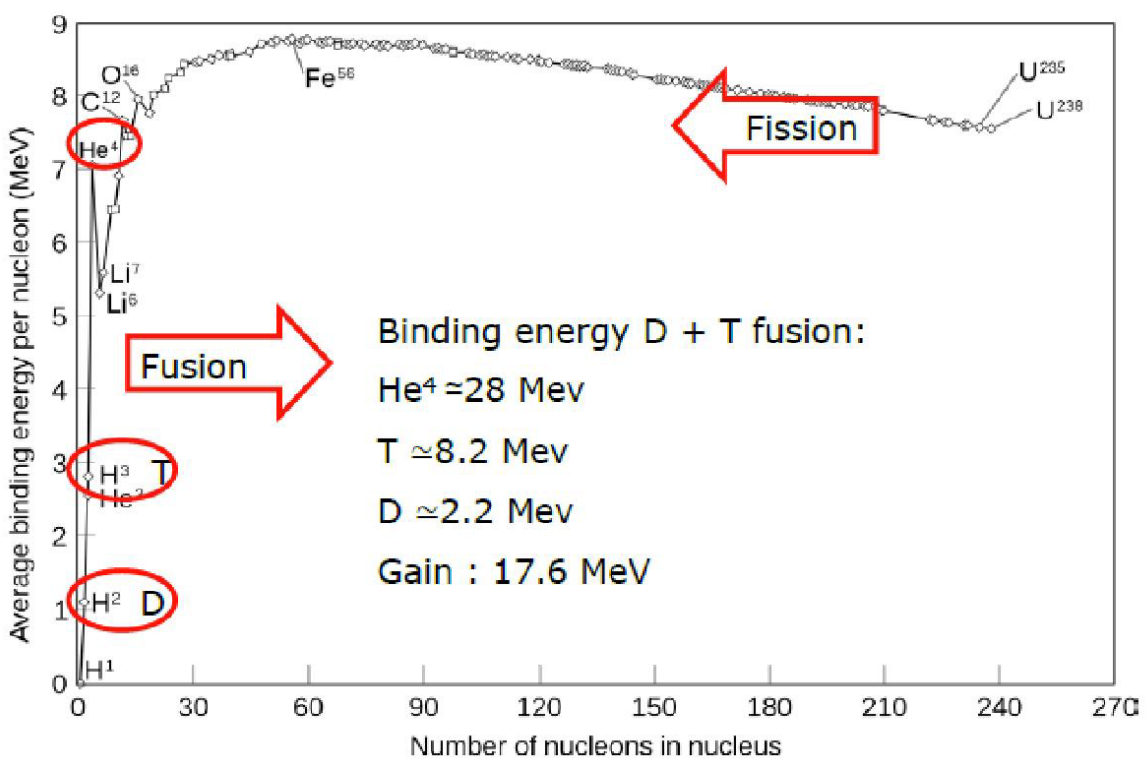
\includegraphics[width=\linewidth]{Chapters/chapter1/figs/binding energy.PNG}
	\caption{Average binding energy per nucleon \cite{YanNingNaulinVolkerWanBaonianXu2014}}
	\label{fig:binding_energy}
\end{figure}

Another factor to consider in comparing different fusion reactions is the likelihood of the reaction to happen. This is characterised by the fusion cross section, which depends on the kinetic energy of the incident particle. Considering an ensemble of particles this kinetic energy translates to temperature. The lower the temperature for which the cross section reaches its peak, and the higher the peak, the easier it is to achieve fusion.
For this and other reasons the reaction that is the main focus of current research is the fusion of deuterium and tritium to helium: \cite{Miley1974}

\begin{equation}
{ }^2_1 D+ { }^3_1T \rightarrow { }^4_2He+{ }^1_0n
\label{eq:fuse}
\end{equation}

In this reaction 3.5MeV kinetic energy is released to the $\alpha$ particle and 14.1MeV to the neutron. Tritium is not available in nature because it is radioactive with a short half life, so it must be produced. It is envisaged that it will be produced using the neutron released in reaction \ref{eq:fuse} in reactions \ref{eq:fuse1} and \ref{eq:fuse2}

\begin{equation}
{}^{6}Li + n \rightarrow {}^{4}He +T +4.78MeV
\label{eq:fuse1}
\end{equation}

\begin{equation}
{}^{7}Li + n \rightarrow {}^{4}He +T +n +2.47MeV
\label{eq:fuse2}
\end{equation}

The initial fuels in this cycle then are deuterium and lithium, both widely available in nature.

\section{Plasma confinement}
%\hl{triple product, H mode, SOL, ELMs}

The temperatures that are relevant for fusion applications are measured in keV, corresponding to millions of °C. At these temperatures matter is in the state of plasma, meaning that atoms are ionised and nuclei and electrons can move freely. These temperatures are of the same order of magnitude as the centre of the Sun. No material can withstand them so special techniques must be adopted to confine the reactant long enough for a significant fraction to fuse. The most important figure of merit of the achieved confinement is the fusion triple product, related to the Lawson criterion, that gives the minimum product of plasma density, temperature and confinement time required to achieve ignition (\autoref{eq:fuse3}). Ignition is the condition when the fusion power output is sufficient to maintain a constant temperature against all losses without external heating.

\begin{equation}
{n_e} {\tau }_{E} T_e  \geq  5\cdot{10}^{21}{ m }^{ -3 }\,s\,keV
\label{eq:fuse3}
\end{equation}

The most viable way to maintain this environment is expected to be
through magnetic confinement fusion (MCF), and specifically the tokamak.
In MCF the fuel is confined in plasma state thanks to its behaviour when exposed to electromagnetic fields. Every electrically charged particle is subject to the Lorentz force:


\begin{equation}
F = q ( E+ v \times B )
\label{eq:lorentz}
\end{equation}

In the presence of a magnetic field the particle gyrates with a circular motion in the direction perpendicular to field lines and is unperturbed in the parallel direction. In a tokamak the plasma is arranged in a doughnut shape, closely surrounded by two main sets of coils. The toroidal field coils generates a magnetic field that is closed in on itself, so that charged particles can be maintained in circular spiralling motion. This toroidal geometry, though, causes an up/down drift in the plasma that would cause it to quickly reach the walls and cool down. This is prevented with a current through the plasma, induced by a central solenoid with a time varying current, that generates the poloidal magnetic field. To further stabilise the plasma and shape it as requested other coils are added to this basic configuration.\cite{Chen1974} The magnetic field generated in this way is composed of concentric flux surfaces expanding out to the coils. The final configuration is outlined in \autoref{fig:mcf}. Shown in pink is a magnetic flux surface, the surface on which a magnetic field line lies. JET is currently the largest tokamak and has achieved triple products higher than $10^{21} m^{-3}\,s\,keV$ in 1997 \cite{Gormezano1998} and recently achieved the record for fusion energy produced, at 59MJ. \cite{Gibney2022}

\begin{figure}[!ht]
	\centering
	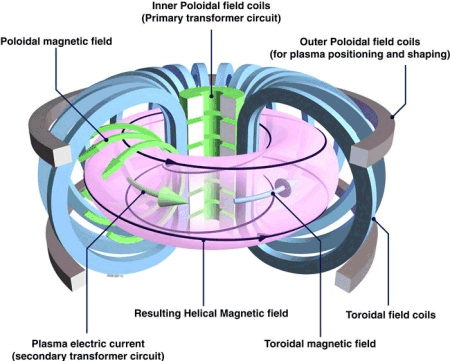
\includegraphics[width=0.7\linewidth]{Chapters/chapter1/figs/mcf.png}
	\caption{Schematic of the main components of a tokamak \cite{CulhamCentreforFusionEnergy2018}}
	\label{fig:mcf}
\end{figure}

The plasma can move freely along the field lines and slowly across it, so in time it drifts from the centre toward the wall via cross field transport caused by collisions and turbulence. One of the important evolutions of the tokamak design is to add a coil parallel to the plasma with a current in the opposite direction. This changes the magnetic configuration in such a way that the core of the plasma is no longer in direct contact with a solid limiter. The first magnetic surface that crosses a solid surface, adjacent the Last Closed Flux Surface (LCFS), is referred as separatrix, and where the poloidal field goes to zero is known as the x-point. The separatrix crosses the solid surfaces in well defined regions, called divertor targets. The plasma that escapes from the core (the position of which is usually referred to as "upstream") reaches the separatrix and then follows the magnetic field around the core and eventually reaches the targets. In this way the core is shielded from the impurities generated by the plasma/surface interaction and can efficiently expel the fusion products. This motion along field lines is much faster than across them and is associated with a layer beyond the LCFS called the Scrape-Off Layer (SOL). The time a particle needs to cross the plasma from the centre and reach the wall defines the confinement time.

\section{H-mode}
A way to limit cross field transport in the core region and move towards ignition is to operate in the so called high-confinement mode (H mode), as opposed to the low-confinement mode (L mode). This regime is reached when the energy flux across the separatrix is increased over a threshold that depends on the discharge conditions.\cite{Ryter1998} The physics behind the specific value of the L-H threshold is still not fully understood, but its effect is to induce a transport barrier at the edge of the core plasma. This barrier strongly reduces the anomalous transport due to turbulence in a thin region around the core, allowing for a better energy and particle confinement there. One drawback of the H-mode is that it causes cycles of accumulation of energy in the core (up to 10\% of the core plasma thermal energy\cite{Zohm1996}) that is then released in sub millisecond bursts of hot plasma. These so called Edge Localised Modes (ELMs) cause a temporary increase of particle and thermal flux on the target of 2-3 orders of magnitude, which is not expected to be tolerable in a large tokamak.\cite{Jachmich2011} The transport barrier is also very effective in confining impurities and fusion products in the plasma core.\cite{Putterich2011} This leads to a dilution of the fusion fuel and a possible radiative collapse of the plasma. ELMs are beneficial in this context as they provide a mechanism to transport impurities across the transport barrier.\cite{Leonard2014}

Various solutions to the ELM problem have been put forward, in the form of different operational regimes where the instabilities that cause the ELMs are prevented or limited, but such solutions usually involve some degree of degradation of the confinement properties typical of the ordinary ELMy scenario, or a limitation of the operational space. Another solution is to 
cause intentionally more frequent and smaller events that can release part of the accumulated energy and particles in a more controlled and gradual manner.\cite{Leonard2014}

In order to sustain the H-mode a certain amount of power must cross the separatrix, otherwise the H-L back transition can occur. This constitutes a lower bound to the heat and particles that need to be dissipated from the separatrix to the target.

\section{The exhaust problem}
%\hl{thin SOL, melting/erosion}

The issue that arises with the divertor configuration is that the SOL is very narrow, of the order of mm\cite{Faitsch2021,Silvagni2020}, and all the exhaust heat is delivered to a small area of the target. For ITER, a fusion device in construction in France that will be a step closer to a power production device, this heat is in the order of $GW/m^2$.\cite{Kuang2020} The maximum power that can be removed from a surface with current technologies is $10-20MW/m^2$.\cite{Pitts2019,Lipschultz2018} If the heat to the target is not mitigated this will pose a serious limitation on its lifetime and the amount of impurities reaching the plasma, making profitable operations impossible. 
Sputtering is the phenomenon of emission of one or multiple atoms from a solid surface caused by interaction with an ion. This happens even for heat fluxes much lower than those required for melting the surface.\cite{Wiesen2017a} There are various types of possible interactions but, as a whole, the larger the energy of the ion, the larger the number of atoms that are sputtered from the surface. The local interaction of the plasma with a solid surface creates a sheath where the ions are accelerated towards the surface, exacerbating sputtering. The flow velocity at the sheath entrance amounts to $v_{se} \geq \sqrt{\frac{kT_e + \gamma kT_i}{m_i}}$ with $m_i$ the ion mass, $k$ the Boltzmann constant, $\gamma=5/3$, $T_e$ and $T_i$ electron and ion temperature respectively, and is higher than the plasma sound speed $c_s \approx \sqrt{\frac{2kT}{m_i}}$. The sputtered atoms can end up in the plasma, polluting it, or be redeposited to the target, changing its composition and properties. Sputtering can be so severe as to be the main limiting factor of the lifetime of the plasma facing components.

\section{Divertor shaping}
%\hl{total/poloidal flux expansion}

The heat and particle flux can be reduced by tilting the target with respect to the separatrix, by locally reducing the magnetic field, thus spreading the heat over a larger surface, and by moving the strike points to a larger radius to spread the heat over a larger surface.
Different divertor designs are under investigation (see some on \autoref{fig:divertor_geometry}) with the purpose, among others, of easing the thermal burden on the target.

\begin{figure}[!ht]
	\centering
	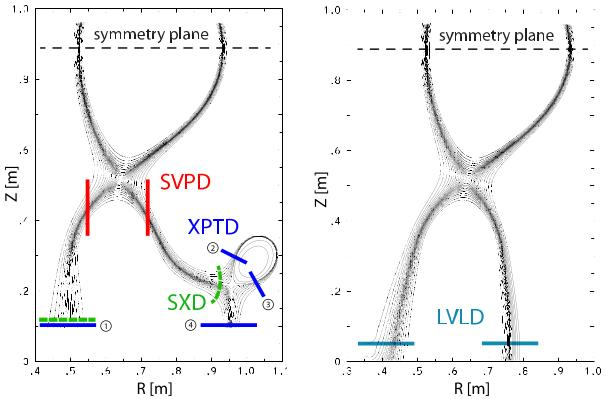
\includegraphics[width=0.8\linewidth]{Chapters/chapter1/figs/divertor geometry.jpg}
	\caption{Example of different divertor configurations. Left: Standard Vertical Plate Divertor (SVPD), Super-X Divertor (SXD) and X-point Divertor (XPTD). Right: Long Vertical Leg Divertor (LVLD) \cite{Umansky2017}}
	\label{fig:divertor_geometry}
\end{figure}

The above mentioned mitigations combined lead to a reduction of the heat flux density of around 20 times for a tokamak of Standard Vertical Plate Divertor (SVPD) divertor type, such as will be implemented on ITER, still short of the additional 10 times reduction needed to respect the $10-20MW/m^2$ limit. The divertor configuration introduces an asymmetry in the toroidal geometry due to the two targets being located at different radii. In terms of energy and particle redistribution in the SOL the inner target will receive a higher ion flux and lower energy flux compared to the outer one. As will become clear later, on the inner target this causes stronger recycling and eases the thermal load, while the outer target is normally subjected to more severe conditions. [\cite{Potzel2014} and references therein]

\section{Radiative dissipation scenario}\label{Radiative dissipation scenario}
%\hl{energy removal --> radiative scenario, impurities}

Another way to decrease the heat flux to the target is to induce radiation in the SOL.
Radiation occurs naturally in plasmas and it depends greatly on the temperature and density of each species. When an atom is not yet fully ionised its electronic levels can be excited by collision and de-excite emitting a photon. The ionised atoms can recombine with free electrons and release a photon too. The energies at which these effects are more likely correspond to the peaks in the curves in \autoref{fig:loss_curve}. If the temperature is so high that atoms are fully ionised, then the only radiative mechanism is Bremsstrahlung radiation that is much less efficient. This corresponds to the monotonically increasing right-hand-side part of the curves in \autoref{fig:loss_curve}.

\begin{figure}[!ht]
	\centering
	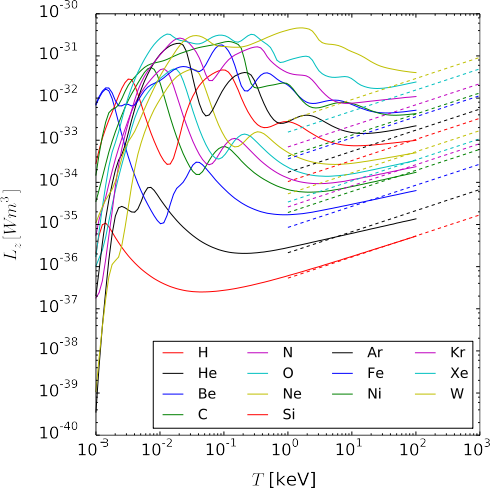
\includegraphics[width=0.7\linewidth]{Chapters/chapter1/figs/loss curve.png}
	\caption{Loss function data from the ADAS data base (solid lines) for the different elements \cite{Lux2015}}
	\label{fig:loss_curve}
\end{figure}

At the temperatures of interest in the SOL (100s of eV\cite{Pacher2011}) hydrogen is fully ionised and radiates weakly. With the addition of impurities sputtered from the wall, or specifically seeded in the discharge, energy can be transferred from the plasma to the impurities and then radiated. This mechanism can be exploited to dissipate a significant amount of power from the core and edge of the plasma, but also the SOL. This regime is referred to as the radiative scenario.


\section{Detachment}\label{Detachment}
%\hl{particle removal -> recycling, detachment}

At low upstream densities the plasma that enters the SOL can flow relatively unimpeded towards the target. The temperature in the SOL is about constant and the particle flux is limited only by the sheath condition (e.g. "sheath-limited"). By increasing the core and SOL density, plasma heat flux conductivity decreases (e.g. "conduction limited"), leading to negative temperature gradients and positive density gradients, with an almost uniform pressure. The heat flux to the target is the sum of the component parallel to field lines $q_{par}$, the orthogonal one $q_{ort}$, and a component given by the energy released with recombination $q_{rec}$, given by  \autoref{eq:detachment}.

\begin{equation}
\begin{aligned}
{ q } _{ par } =& { n } _{ e,t } { c } _{ s } {  \gamma  } _{ sh }{ k } _{ B }{ T } _{ e,t } \; \alpha \; { p } _{ e,t }{{ T } _{ e,t }}^{0.5 } \\
{ q } _{ ort } =& { q } _{ par } \left( \frac {{ B } _{ p }} {{  B  }_{ \phi  }}   \right) _{ t} \; \alpha \; { p } _{ e,t }{{ T } _{ e,t }}^{0.5 } \\
{ q } _{ rec } =& { n } _{ e,t } { c } _{ s } {  E  } _{ pot } \; \alpha \; { p } _{ e,t }{{ T } _{ e,t }}^{-0.5 }
\end{aligned}
\label{eq:detachment}
\end{equation}

where $\gamma_{sh}$ is the heat sheath transmission factor, $n_{e,t}$ and $T_{e,t}$ are the electron density and temperature in front of the target, $c_s$ is the sound speed, $B_p$ and $B_{\Phi}$ are the poloidal and toroidal magnetic fields and $E_{pot} \approx 15.8 eV$ is the potential energy released per ion when recombining to form neutral deuterium molecules on the target plate. \cite{Reimold2015} The temperature cannot be indefinitely reduced because of operational limits such as the Greenwald limit.\cite{Greenwald1988} Moreover, a reduction of the temperature does not alone guarantee a decrease of the heat flux.  One possible solution to achieve it is to cause gradients of temperature and pressure along the field lines in the SOL. This should be done in such a way to minimize the impact on the core plasma.

A way to achieve this is to induce plasma detachment. This phenomenon has been observed in a series of tokamaks [\cite{Reimold2015} and references therein] and can be induced by impurity seeding or fuelling. In Alcator C-Mod \cite{Lipschultz2007} and AUG \cite{Kallenbach2015a} it was shown to significantly reduce target heat flux in conditions scalable to burning plasmas like ITER.

In an attached regime the plasma streams through the SOL and reaches the target. At the target the charged particles recombine and become neutrals. These are generated in an excited state and, therefore, there is strong radiation at the strike points. The neutrals are not bound by magnetic fields and can move freely until they collide with other neutrals or particles from the plasma. A neutral can then re-ionise and stream along field lines, returning to the target or entering the plasma again. This process is called recycling and the region of the leg where it occurs is called the ionisation or recycling region.

If the density in the SOL is high enough then the neutrals generated at the surface by the plasma will interact mainly in the SOL and the plasma will lose part of its energy and momentum on its way to the target via radiation and transport.\cite{Leonard2018} To further increase the energy loss, low Z impurities like Nitrogen can be seeded in the SOL: they will ionise only partially, radiating efficiently at a higher temperature than hydrogen or helium. The lower the temperature, the higher the energetic ionisation cost will be. This is because lower temperature means slower progressive excitation by collisions of the bound electron up to ionisation, with radiative losses in the process, instead of a single higher energetic collision directly to ionisation. This causes even more radiative cooling. In most cases volumetric ionisation from neutrals constitutes the main source of ions for the target flux. This effect is even stronger if the divertor is separated from the main chamber by a physical barrier, the baffle, that confines the neutrals increasing their density in the divertor, like in the Mega Amp Spherical Tokamak Upgrade (MAST-U) tokamak. \cite{Krasheninnikov2016,Krasheninnikov2017a,Lipschultz1999} This is referred to as high recycling, where the recycling region constitutes a self-contained system that is supplied from upstream with the energy to ionise the neutrals. This is believed to be one of the most important differences between tokamak divertors and linear machines, where the main source of ions is usually the plasma source upstream. Simulations for the linear machine Pilot-PSI, characterised by a very high density, show that ionisation could account for up to a third of the plasma source, but in a region very close to the source itself.\cite{Jesko2018,Hayashi2016}

From detachment experiments it is observed that the particle flux to the target increases with increasing core density. Increasing the density or seeding impurities causes the particle flux to reach a maximum and then decrease. This is called rollover and corresponds with the onset of detachment. Other metrics for detachment onset have been used, such as the decrease of the target temperature below a certain threshold\cite{Stangeby2000,Goldston2017}, but the Langmuir probe particle flux roll over constitutes a direct and simple measurement, hence their widespread use. Further increasing the density the particle flux decreases and saturates. In the case that the plasma loses all its kinetic or thermal energy it still maintains the energy absorbed during its creation, the ionisation and dissociation energy, $15.8eV$. In a DEMO scale device this residual energy flux would be still high enough to exceed the $10-20 MWm^{-2}$ limit on the target. \cite{Krasheninnikov2017a} To reduce it even further the temperature must drop below $1eV$ to trigger volumetric recombination. This is accompanied by a strong radiation increase from where volumetric recombination occurs. The particle flux drop can continue up to the point that the measured plasma temperature at the target reaches a minimum and the radiating region (radiation front) recedes upstream along the field lines.\cite{Krasheninnikov1999} At different stages in this process different fronts will in turn detach from the target like the ionisation and thermal front.\cite{Hutchinson1994,Loarte1998,Lipschultz2016} The front's movement comes from the balance between the power and particles entering the SOL with dissipation by radiation and interaction with recycling neutrals.


% \section{Atomic and molecular processes}
% \hl{
%             1. attached $->$ hot $->$ atomic physics
%             2. detached $->$ cold $->$ atomic and molecular physics}


\section{The x-point radiator}\label{The x-point radiator}
%\hl{extreme end of detachment before MARFE, increased radiated power}

When a discharge, either L-mode or H-mode, is close to the detachment threshold in a tokamak with a conventional divertor configuration, and the impurity or core density is increased, 4 stages of detachment are defined as per the description in \cite{Reimold2015,Potzel2014} (here detachment is intended to mean the particle flux roll over and deviation from what is expected in the attached case, see \autoref{Analytic models}).

\begin{enumerate}
    \item Onset of detachment: the inner target detaches inter-ELMs (both from impurity seeding and from upstream density increase), the outer target is attached
    \item Fluctuating state: radiative fluctuations (of order kHz) appear at the X-point, inner target detaches inter-ELMs
    \item Partial detachment at outer target: inner target always detached, outer target detached inter-ELMs, strong radiation at the X-point, fluctuations frequency decrease to ELMs scale, ELM's amplitude decrease.
    \item Complete detachment: inner and outer target always detached, sporadic ELMs, radiator moves from X-point further into the confined plasma
\end{enumerate}

For this type of discharge the radiator close to the X-point appears when detachment starts at the inner target, while it is only enhanced by the detachment on the outer target. Because the parameter of interest is the reduction of thermal flux on the outer target, a feature that will always be present in reactor relevant conditions is a strong radiator located close to the X-point.

If the density is further increased, the radiator can either move vertically upwards entering the core\cite{Bernert2021}, or move along the inner separatrix up to the midplane and enter the core from there.\cite{Lipschultz1984} In both cases a degradation of the confinement properties is observed.

\section{Effect of X-point radiator}\label{Effect of X-point radiator}
%\hl{poloidal asymmetry, pedestal flattening, loss confinement}


The X-point radiator (XPR)\cite{Bernert2021} or X-point MARFE\cite{Kallenbach2015a} is a region of steep temperature gradient, where the temperature goes from that of the hot upstream plasma from the core to the cold region where ion / neutral interactions dominate. The presence of such a region at or inside the separatrix can lead to confinement degradation. In this context, what is referred to as confinement H98 is the ratio of the actual energy confinement time $\tau_{th}$ to a reference. The reference is a confinement time from a scaling law obtained by fitting the confinement time of many tokamak experiments in a certain operating mode. For ELMy H-mode the scaling law mostly used is the ITER Physics Basis (IPB) 98(y,2).\cite{Doyle2007} For L-mode the ITERL-97P scaling can be used. \cite{Kaye1997} The scalings are given by \autoref{eq:h98y2} and \ref{eq:l97}. For spherical tokamaks an H-mode \cite{Kaye2006} and MAST L-mode \cite{Kaye2021} scaling are given in \autoref{eq:HST}, \ref{eq:LST} respectively


\begin{equation}
{ H }_{ 98 }={\tau }_{ th }/{\tau }_{ th,98y2 } \; , \; {\tau }_{ th,98y2 }=0.0562 {{ I }_{ P }}^{ 0.93} {{ B }_{ t }}^{ 0.15} {{ n }_{ 19 }}^{ 0.41} {{ P }_{ L }}^{ -0.69} {{ R }_{  }}^{ 1.97} {{ \varepsilon  }_{  }}^{ 0.58} {{ \kappa  }_{ a }}^{ 0.78} {{ M }_{  }}^{ 0.19}
\label{eq:h98y2}
\end{equation}

\begin{equation}
{ L }_{ 97 }={\tau }_{ th }/{\tau }_{ th,97P } \; , \; {\tau }_{ th,97P }=0.037 {{ I }_{ P }}^{ 0.74} {{ B }_{ t }}^{ 0.2} {{ n }_{ 19 }}^{ 0.24} {{ P }_{ L }}^{ -0.75} {{ R }_{  }}^{ 1.69} {{ \varepsilon  }_{  }}^{ 0.31} {{ \kappa  }_{ a }}^{ 0.67} {{ M }_{  }}^{ 0.26}
\label{eq:l97}
\end{equation}


\begin{equation}
{ H }_{ ST }={\tau }_{ th }/{\tau }_{ th,HST } \; , \; {\tau }_{ th,HST }=0.066 {{ I }_{ P }}^{ 0.53} {{ B }_{ t }}^{ 1.05} {{ n }_{ 19 }}^{ 0.65} {{ P }_{ heat }}^{ -0.58} {{ R }_{  }}^{ 2.66} {{ \kappa  }_{ a }}^{ 0.78}
\label{eq:HST}
\end{equation}

\begin{equation}
{ L }_{ ST }={\tau }_{ th }/{\tau }_{ th,LST } \; , \; {\tau }_{ th,LST }=0.153 {{ I }_{ P }}^{ 1.01} {{ B }_{ t }}^{ 0.7} {{ n }_{ 19 }}^{ -0.07} {{ P }_{ L }}^{ -0.37}
\label{eq:LST}
\end{equation}

with $I_P$ plasma current in $MA$, $B_t$ toroidal magnetic field in $T$, $n^{19}$ averaged electron density in units of $10^{19} \#/m^3$, $P_L=P-dW/dt$ power loss in $MW$ with $P$ heating power and $W$ stored energy, $R$ major radius, $a$ minor radius, $\varepsilon=a/R$ inverse aspect ratio, $\kappa _a$ elongation, $M$ ion mass number in $amu$.
It is possible to calculate the energy confinement time from magnetic coil measurements and the energy transferred to the plasma as heating ($P_{heat}$). $\tau_{th}$ is defined by 

\begin{equation}
\begin{split}
\frac {dW} {dt}={P}_{heat} - \frac {W} {\tau }_{ th } \; , \; W=\frac { 3} {2} \langle p \rangle V \; , \; \langle p \rangle = \frac {{ \mu }_{ 0 } {{ I }_{ p }}^{ 2 } { \beta }_{ p }} { 8 {\pi}^{2} {a}^{2}  } \\ {\beta }_{ p } = \langle \frac { n {k}_{B} T} { {{B}_{p}}^{2} /(2 {\mu}_{0}) } \rangle \; , \; {P }_{ heat }={ P }_{ ohmic }+{ P }_{ NBI }+{ P }_{ RF }
\label{eq:tau}
\end{split}
\end{equation}


With $V$ plasma volume, $\langle p \rangle$ volume-averaged plasma kinetic pressure, ${{ \beta }_{ p }}$ poloidal beta, $B_p$ poloidal magnetic field, $a$ minor radius, $P_{ohmic}$, $P_{NBI}$, $P_{RF}$, power transferred to the plasma by ohmic heating, neutral beam injector and radio frequency respectively. \cite{SalarElahi2010,Wesson2011} The confinement loss is usually determined by comparing the confinement before and after the appearance of the X-point radiator, or by comparing a series of discharges in similar conditions with and without X-point radiator.
The confinement degradation can be due to direct cooling caused by the cold region (e.g.poloidal temperature gradients driving power to that location \cite{Lipschultz1998} ) or to easier penetration of impurities in the core [\cite{Lipschultz2016} and references therein]. The degradation significantly affects the outer part of the core region with significant reduction of temperature, pressure and an increase in density. \cite{Kallenbach2015a}  It was found on some experiments that the inner core (i.e. where the ratio of poloidal magnetic flux over poloidal magnetic flux at the separatrix $ \rho _{pol}<0.8-0.5 $) is only marginally effected. [\cite{Reinke2013} and references therein] It is therefore suggested that the reduction of the gradients in the pedestal region could be recovered in a portion of plasma $0.8< \rho _{pol}<0.95$. \cite{Reimold2015}

The X-point radiator will also have the effect of radiating a substantial fraction ($75-90\%$ of the heating power achieved \cite{Bernert2017}) of the power input to the core. This could reduce the power crossing the separatrix, causing the H-L transition. This is not a major risk for ITER and larger machines, because the power crossing the separatrix is expected to be significantly larger than the threshold requirement. In fact, seeding a higher-Z impurity into the plasma to enhance core radiation (radiative mantle) and lower the power needed to be exhausted through the separatrix to about the minimum for the L-H transition, has been considered. Then a lower-Z impurity will be fed to radiate in the divertor. [\cite{Kallenbach2015a,Reinke2013} and references therein]


There are two active areas of research to limit confinement losses with XPR.

One is in trying to achieve detachment while not allowing the radiator to move all the way to the X-point and cause confinement degradation. The main difficulty in achieving this is that, for standard divertor geometries, the operational window of any given control parameter to move the radiator from target to X-point is very narrow. Considerable effort has been put forward to find a predictive model. An early attempt is the two point model, a 1D model where the conditions outside the separatrix and at the target are correlated and some approximations on the heat and particle transport adopted.\cite{HOBBS1966,Hobbs1967,Mahdavi1981,Keilhacker1982,Harbour1984,Lackner1984,Stangeby2001} The thermal front model proposed by Lipschultz \cite{Lipschultz2016} is an improved 1D model that, balancing input / output power on the thermal front (edge of the radiator toward the core), tries to identify the operational window of a control parameter and its stability for given plasma / magnetic configuration. This model finds that for all the control variables analysed, the operational window widens for an increasing ratio of X-point to target magnetic field $B_x/B_t$; and increasing ratio of the connection length between X-point and target to upstream and target $z_X/L$. It is also found that increasing connection length should lower the detachment upstream density threshold. Stability analysis indicates that for decreasing $z_X/L$ there is an increasing minimum Bx/Bt for a stable solution.\cite{Lipschultz2016}

This puts additional emphasis on research of different divertor designs. TCV in Switzerland and MAST-U in UK are the best suited for these type of investigations due to the flexibility of their divertor geometry. Recent data from TCV seems to prove that the sensitivity on control parameters decreases with flux expansion (larger operational window) but didn’t verify the threshold dependence on connection length. \cite{Theiler2017}

A second strategy is to live with the radiator located at the X-point (it is further apart from the target and ELMs have to burn through more divertor volume before reaching the target) and try to understand and minimize the loss of confinement in the core. The reality of current conventional tokamaks is that the X-point radiator always appears if full detachment from the target is pursued, with different variations depending on the seeded impurity as can be seen in \autoref{fig:xprs}.

\begin{figure}[!ht]
	\centering
	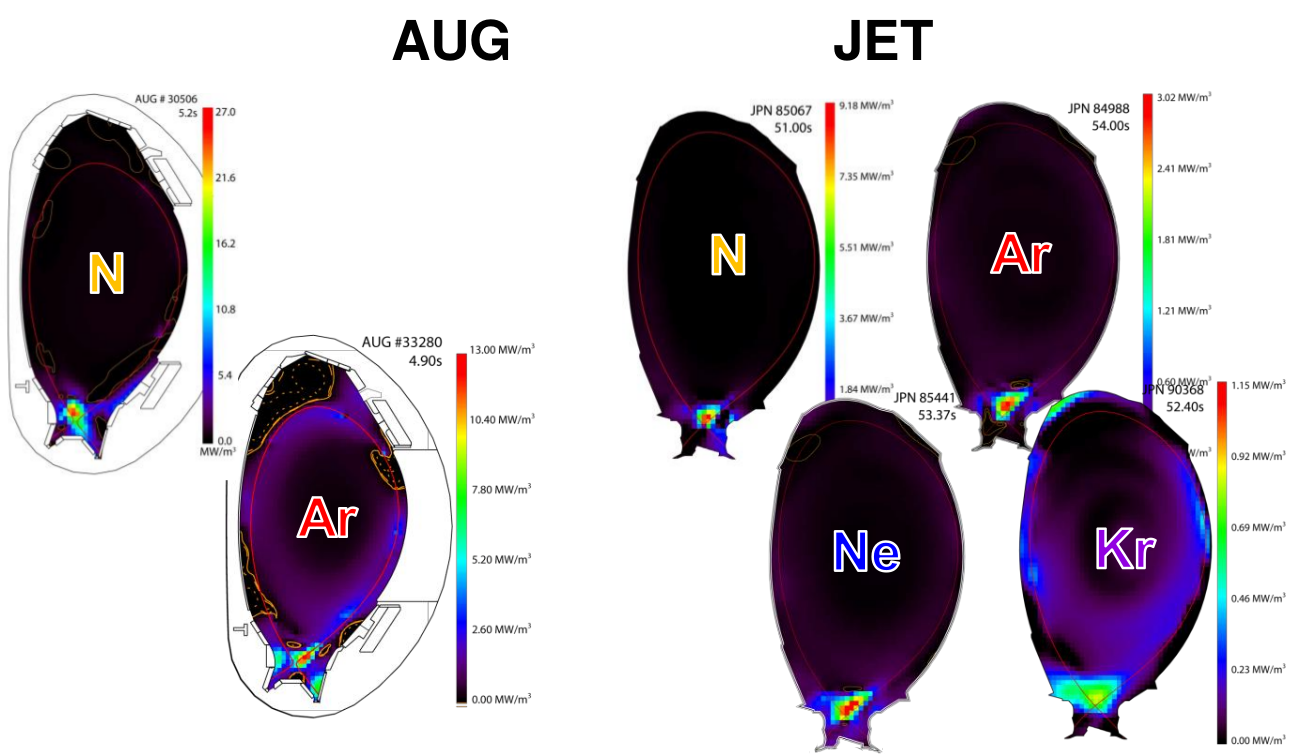
\includegraphics[width=\linewidth]{Chapters/chapter1/figs/xprs.png}
	\caption{Different radiation profiles with the clear presence of an X-point radiator for different impurities
	\cite{Wiesen2017}}
	\label{fig:xprs}
\end{figure}

The X-point radiator cannot be idealised as easily as the thermal front of detachment, because it is much more related to core and edge dynamics. Modeling its behaviour requires the use of codes that account for all atomic interactions, drifts, etc. such as SOLPS-ITER, EDGE2D-EIRENE, SOLEDGE2D-EIRENE [\cite{Wiesen2017a} and references therein]. The presence of the radiator significantly affects temperature, pressure and density distribution, especially in the pedestal, therefore it is likely to have an effect on the current distribution and MHD activity.
In recent years a large effort has been put forward to characterise the behaviour of the X-point radiator and its macroscopic effects on the core / edge. This has been done mostly in conventional geometry tokamaks, both with metal and carbon walls.


\section{ELMs and XPR}
Another important feature of the XPR is the reduction in amplitude of ELMs. This can be attributed to the fact that the energy associated with an ELM first heats up the XPR and then moves toward the target. If the neutral density between the X-point and target, and in the radiator itself, is high enough then it could be possible to avoid ELM “burn through”, where the ELM penetrates the detachment front and reaches the target. \cite{Krasheninnikov2016} This can be further improved by alternative divertor configurations, like the super-x divertor with a long outer leg, since the ELM has more time to interact the cold gas and dissipate some of its energy. The burn through is a complex phenomenon because of the short time scale (hundreds of $\mu s$), complex geometry and complex interactions between the core plasma being expelled by the ELM with the neutrals.

Simulations with simplified atomic and neutral physics have been carried out with the code JOREK to study the dynamic of the burn through in MAST-U, showing a significant reduction of the peak target heat flux compared to empirical scalings.\cite{Smith2020,Smith2020a} Other attempts with the code SOL-KiT have shown the importance, given the short time scale of the burn through, of including kinetic effects and that the target flux could be underestimated with fluid models.\cite{Mijin2020}
Attempts to better the understand the physics of detachment and the burn through with a more detailed model that includes molecular reactions with simpler geometric approximations (SD1D) have revealed that molecular reactions are important for the plasma momentum balance and cause Balmer $\alpha$ radiation to increase at and after the roll over.\cite{Zhou2022} 
These attempts could recreate target power fluxes similar to experiments, but require significant refinement to return sensible results.\cite{Tskhakaya2009} No simulation yet, to the knowledge of the author, includes a complete treatment of the molecular reactions that become relevant at the low temperatures typical of deep detachment ($<5eV$) together with the 3D and kinetic effects that have been shown to be important.

\section{Analytic models}\label{Analytic models}

In order to qualify and characterise the evolution of detachment it is useful to build approximate analytical models for the properties of interest, like particle and power fluxes, depending on the upstream plasma conditions. The most widely model is the two point model (2PM) and its variations.\cite{HOBBS1966,Hobbs1967,Mahdavi1981,Keilhacker1982,Harbour1984,Lackner1984,Stangeby2001} In it the complex 3D geometry of the SOL is translated to a simpler 1D system as shown in \autoref{fig:2PM}.

\begin{figure}[!ht]
	\centering
	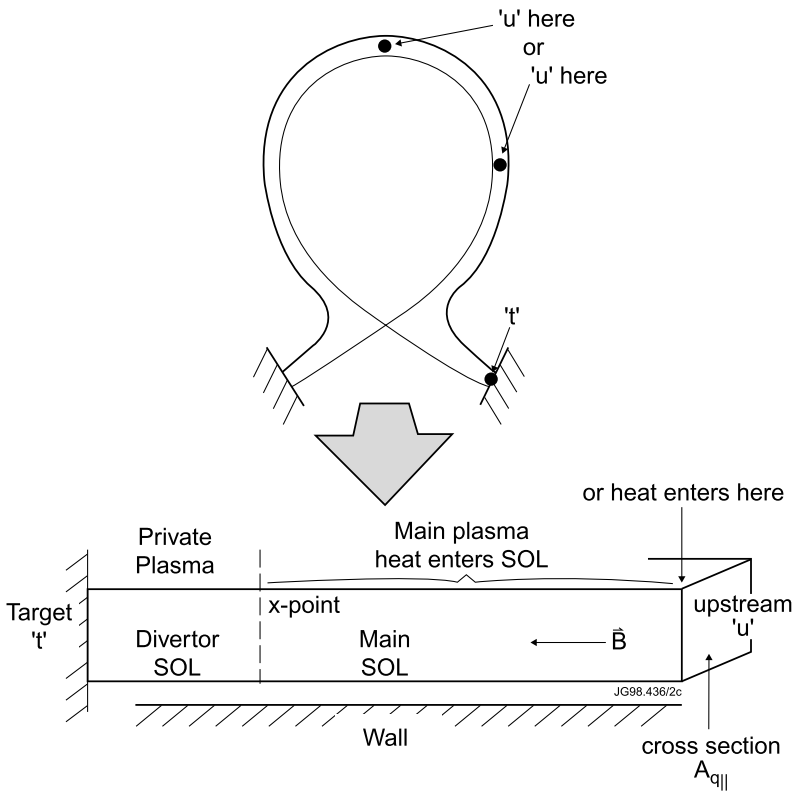
\includegraphics[trim={0 0 0 0},clip,width=0.65\linewidth]{Chapters/chapter1/figs/2PM.png}
	\caption{Schematic of how the poloidal SOL geometry can be straightened into a 1D one. 'u' indicates the location of the upstream location where core plasma enters the SOL.% The model is weakly sensitive to the location of the upstream location, assuming gradients are weak far from the divertor.\cite{Verhaegh2018} 
     Adapted from \cite{Harrison2011} and the JET image database.}
	\label{fig:2PM}
\end{figure}

Then a series of assumptions are made:
\begin{itemize}
    \item there are no power losses along the SOL%, excluding all radiated power losses
    \item ionisation does not affect the energy and flow profile
    \item heat is transported only via parallel heat conduction
    \item plasma pressure is considered constant in the entire SOL
    \item quasi neutrality, and the same temperature for electrons and ions ($n_e = n_i = n$, $T_e = T_i = T$)
    \item all the power to the SOL is transferred at the upstream location.
\end{itemize}

At the target surface the presence of the sheath accelerates the ions to the sound speed, so the local pressure given by the static and dynamic component $p_t$ is

\begin{equation}
p_{t} = p_{static} + p_{dynamic} = 2n_{t} k T_{t} + n_{t} m_i {{c_s}_t}^2
\label{eq:2pm1}
\end{equation}

Upstream, the velocity component of the pressure is assumed to be negligible so, $p_u \approx 2 n_u k T_u$, so that if the pressure is considered uniform then this returns the first equation of the 2PM

\begin{equation}
2 n_u k T_u = 2n_{t} k T_{t} + 2n_{t} k T_{t} \rightarrow n_u T_u = 2n_{t}T_{t}
\label{eq:2pm2}
\end{equation}

Since no volumetric power loss is considered, the heat transferred to the SOL is transported to the target, and it is determined by the sheath physics to be

\begin{equation}
q_{\parallel} =  \gamma n_t k T_t {c_s}_t = \gamma n_t \sqrt{\frac{2(kT_t)^3}{m_i}}
\label{eq:2pm3}
\end{equation}
returning the second equation of the 2PM.

This heat is carried to the target via conduction. In order to calculate it, using Spitzer conductivity\cite{Stangeby2001}, one should consider that the parallel heat conductivity for charged particle self-collisions can be written as ${v_{th}}_s \lambda_s \approx {{v_{th}}_s}^2/{\nu_s}$ with ${v_{th}}_s$ the unidirectional thermal velocity of the species $s$, $\lambda_s$ the self-collision mean free path and $\nu_s$ the self-collision frequency. ${v_{th}}_s$ is given by $\sqrt{8kT_s/{m_s}}$ while $\nu_s$ is proportional to $n_s/\sqrt{m_s T_s^3}$. The heat conductivity is then proportional to $ {T_s}^{5/2} / {m_s}^{1/2}$. This indicates that, given the mass difference, electrons dominate the conduction heat transfer, and that there is a strong dependency on the temperature. The heat flux can then finally be written as per \autoref{eq:2pm4a} where the electron parallel heat conductivity coefficient $\kappa$ is of the order of 2000.\cite{Stangeby2001}

\begin{equation}
q_{\parallel} = -\kappa T^{5/2} \frac{dT}{ds_{\parallel}}
\label{eq:2pm4a}
\end{equation}

This equation can be integrated from upstream to target (amounting to the connection length $L$), and considering that $q_{\parallel}$ is constant one can obtain the last equation of the 2PM model

\begin{equation}
{T_u}^{7/2} = {T_t}^{7/2} + \frac{7 q_{\parallel} L}{2 \kappa}
\label{eq:2pm4}
\end{equation}

Assuming fixed $q_{\parallel}, L, \gamma, m_i$ \autoref{eq:2pm2}, \ref{eq:2pm3} and \ref{eq:2pm4} contain 4 unknowns ($n_t, n_u, T_t, T_u$) and can be used to numerically solve for 3 when one is known or measured. If one assumes $T_u >> T_t$ %as it is the case in the conduction limited regime, 
\autoref{eq:2pm4} can be further simplified neglecting $T_t$ and the 2PM reduces to

\begin{equation}
\begin{aligned}
T_t =& \frac{{q_{\parallel}}^2}{{n_u}^2 {T_u}^2} \; \frac{2m_i}{\gamma^2} \\
n_t =& \frac{{n_u}^3 {T_u}^3}{{q_{\parallel}}^2} \; \frac{\gamma^2}{4m_i} \\
T_u =& \left( \frac{7 q_{\parallel} L}{2 \kappa} \right)^{2/7}
\end{aligned}
\label{eq:2pm5}
\end{equation}

The target particle flux can finally be calculated as the heat flux over the energy released by each particle (neglecting the energy from surface recombination) from \autoref{eq:2pm3} as shown in \autoref{eq:2pm6} (the arrow refers to the further simplification as per \autoref{eq:2pm5}).

\begin{equation}
\Gamma_t = \frac{q_{\parallel}}{\gamma T_t} =  n_t \sqrt{\frac{2kT_t}{m_i}} \rightarrow \frac{{n_u}^2 {T_u}^2}{q_{\parallel}} \; \frac{\gamma^2}{2m_i}
\label{eq:2pm6}
\end{equation}
This correlation is the one that has been used in the literature to find detachment. The particle flux from Langmuir probes and the expectation from this scaling roughly match for an attached target. Increasing the upstream density further, the particle flux plateaus and then starts to decrease, deviating from the expected trend. This can be quantified in the Degree of Detachment (DoD) given by the ratio of the two quantities.\cite{Stangeby2001,Loarte1998}

This simple model can then be improved by including more of the true physics of the divertor and SOL such as: volumetric power and momentum losses due to interactions with neutrals, volumetric radiated power losses, variation in $q_{\parallel}$ and pressure along field lines, sharp transition regions from x-point to target (e.g. ionisation / density / radiation front), magnetic configuration, etc.\cite{Stangeby2001,Cowley2022,Reinke2017,Lipschultz2016} This increase of sophistication also allows, depending on the model, the study of the conditions along the leg, and investigation of the relevance of different phenomena and the stability of the front's movement. The front's stability is particularly important because, as detached scenarios become more and more relied upon to provide the volumetric dissipation required for the target survival, it is paramount to be able to control their location. It has also been demonstrated that the threshold for rollover is proportional to a certain value of the ratio $ \frac {q_{rec}} {p_{up}}$ ($q_{rec}$ is the specific energy flux into the hydrogen recycling region). \cite{Krasheninnikov1999,Krasheninnikov2016,Stangeby2018}

Of relevance for the present work is that the depth of detachment increases with upstream density. This will be used to characterise density ramps in MAST-U during the first experimental campaign (MU01).

\section{Goals and objectives of the thesis}

The main objective of this work is an understanding of the radiation distribution on MAST-U and its relation to detachment. This is achieved with the design, implementation, calibration, validation and use of  the new infra-red video bolometer diagnostic in MAST-U. As will be shown in detail in \autoref{chapter2}, the diagnostic is based on previous work on NSTX-U\cite{VanEden2016} and Alcator C-Mod\cite{Reinke2018a} and its goal is to measure the radiation distribution in the lower section of MAST-U with particular emphasis on the x-point region.

Significant work was necessary to design the system and to balance the strength of the signal with the desire to maximize spatial resolution (see \autoref{MAST-U IRVB design}). For this, new and accurate ray tracing methods were used in order to accurately determine the intensity of the radiation from the plasma on the diagnostic.

Once the diagnostic was built it was necessary to calibrate it in order to convert the data to a form related to the power radiated by the plasma (see \autoref{System calibration}). This was done by characterising all parts of the diagnostic and by finally verifying its accuracy compared to a known source. Once installed on MAST-U the orientation and the field of view was verified using features of the plasma, obtaining good agreement with the original design.

Finally the data from MAST-U is collected and analysed (see \autoref{MU01 Line integrated results}). The changes of line integrated brightness in different region of the plasma correlated well with the progress of detachment. The measurements match observations from another diagnostic that observes the total radiated power (the resistive bolometry system), albeit being negatively effected by imperfections in the sensing element and a signal from the NBIs unrelated to the radiated power effecting part of the field of view.

In parallel to the hardware development, an effort was made to develop inversion routines capable to tomographically invert the line integrated brightness to emissivity (see \autoref{Inversion techniques}). Different methods were tested and a probabilistic approach was adopted to take into account the uncertainties arising from the different parts of the system.

The results show, for the first time in a spherical tokamak, the changes of radiation distribution in relation with detachment with high spatial resolution (see \autoref{MU01 tomographycally inverted results}). The movement of the radiation in the inner and outer leg can be compared with literature\cite{Reimold2015,Potzel2014,Lipschultz1984,Bernert2021} and it is found that the progression is similar to expectations for L-mode, while it was not in the H-mode discharges. The progress of detachment in L-mode is compared to measurements from other diagnostics. The particle flux on the outer target is observed to consistently roll-over after the radiation is detached on the inner target and at the same time as the outer target radiatively detaches.
The radiated power in the core region scales well with measurements from the resistive bolometry system while the total power radiated in the super-x chamber is used in conjunction with measurements of the hydrogen and carbon line emission to confirm recent results on the processes involved with detachment\cite{Verhaegh2022} and the importance of molecular assisted reactions as an intermediate step between electron impact ionisation and electron-ion recombination.

A secondary goal of this work, developed thanks to a collaboration with the DIFFER institute in The Netherlands, is understanding the behaviour of ELM-like pulses during detachment and the role of atomic and molecular processes. This was achieved by conducting a series of experiments on the linear plasma machine Magnum-PSI, and upgrading the existing optical emission spectrometer to operate intra-shot measurements, as detailed in \autoref{chapter3}.

Conditions similar to the end of a target in a tokamak were reproduced, changing the neutral pressure to cause the target to transition from attached to detached. Superimposed on this steady state regime, ELM-like pulses are recreated with a dedicated power supply system. These is a sudden increase of the plasma temperature and density such that the heat flux increases transiently by 1 order of magnitude. Temporally and spatially resolved measurements are taken with different diagnostics to understand the burn through process. This is difficult to do in a tokamak because of poor diagnostic access and reproducibility.

Direct measurements from a fast camera observing the burn through process tangentially and an infrared camera observing the target are used to determine that, when the neutral pressure is sufficiently high, the ELM-like pulse is prevented from effecting the target and the plasma is dissipated in the volume instead.

The measurements from the optical emission spectrometer were used in conjunction with other diagnostics to build a Bayesian algorithm capable of inferring the most likely properties of the plasma, poloidally and temporally resolved. This is used to show, similarly to what was done in the study on MAST-U, the importance of molecular assisted reactions. Molecular processes are important in the exchange of potential energy, while less so in radiating the energy from the ELM-like pulse. It is also found that, for some conditions, the volumetric ionisation source is more important than the plasma input from the source, making these conditions closer than other linear machines to what observed in tokamaks.


% \subsection{XPR/radiation front location and confinement (maybe the dataset is not there)}
% find limit where confinement is not compromised, correlation between confinement and XPR/radiation location
% \subsection{poloidal (toroidal?) divertor after XPR}
% radiation spreading over all the separatrix, trasforming it into a limiter for the plasma.
% \hl{I never observed this, is it worth mentioning?}
% \subsection{XPR/detachment and power balance}
% radiator location vs radiated power
% \subsection{radiation front location and analytic models}
% DOD vs radiator location, radiation front range/stability vs prediction
% % \subsection{detachment and configuration (CD/SXD)}
% % radiated power vs configuration (against predictions)
% \subsection{radiation location and other metric of detachment}
% radiator location vs MWI/LP compared to expectations, ionisation/MAR/recombination region (Kevin work)
% % \subsection{XPR and ELMs}
% % ELMs burn through/impact on LP and IR vs detachment/radiation front location
% % \subsection{Cyd Cowley paper}
% % hysteresis in inner leg detachment
% \subsection{ELMs baffled in linear machine}
% Magnum work, it is possible to prevent ELMs to reach the target with target pressure
% \subsection{atomic vs molecular effects during ELMs burn through in deep detachment in linear machine}






